\documentclass[12pt]{amsart}
\usepackage[letterpaper, portrait, left = 1in, right = 1in, top = 1.2in, bottom=1.5in]{geometry} 
%\usepackage{setspace} \doublespacing
%\usepackage[letterpaper, portrait, margin=1.3in]{geometry}
\usepackage[table,xcdraw]{xcolor}
\usepackage{amssymb}
\usepackage{amsfonts}
\usepackage{longtable}
\usepackage{amsmath,amsthm}
\usepackage{enumitem}
\usepackage[utf8]{inputenc}
\usepackage{mathtools}
\usepackage{graphicx}
\usepackage{parskip}
\usepackage{multicol}
\usepackage{listings}
\usepackage[skip=0.25pt]{caption}
\usepackage[mathscr]{euscript}
\usepackage{quiver}
\setlength{\parindent}{0pt}
\usepackage{thm-restate}
\definecolor{vividburgundy}{rgb}{0.62, 0.11, 0.21}
\usepackage[driverfallback=hypertex,pagebackref=false,colorlinks,citecolor=vividburgundy]{hyperref}
\usepackage[capitalize]{cleveref}
%\usepackage[cmintegrals,cmbraces]{newtxmath}
%\usepackage{ebgaramond-maths}

%\usepackage{fourier}
%----------FONT OPTIONS----------
% sans-serif
%\usepackage[sfdefault]{FiraSans}
 %\usepackage[sfdefault]{roboto}
% \usepackage[sfdefault]{noto-sans}
%\usepackage[default]{sourcesanspro}

% serif
%\usepackage{CormorantGaramond}

%\usepackage{charter}
\usepackage[T1]{fontenc}
\usepackage{cleveref}
\definecolor{dg}{RGB}{10, 100, 10}
\setlength{\parindent}{0in}
\renewcommand{\qed}{$\hfill\blacksquare$}
% \newtheoremstyle{style}{2pt}{1pt}{\normalfont}{}{\bfseries}{\\}{0cm}{}
% \theoremstyle{style}
\newtheorem{lemma}{Lemma}[section]
% \newtheorem{lemma}{Lemma}
\newtheorem{thm}[lemma]{Theorem}
\newtheorem{prop}[lemma]{Proposition}
\newtheorem{cor}[lemma]{Corollary}
\newtheorem{conj}[lemma]{Conjecture}
\newtheorem{cl}[lemma]{Claim}
\newtheorem{rmk}{Remark}
\newtheorem{defn}[lemma]{Definition}
\newtheorem{qs}{Question}
\newtheoremstyle{styleS}{}{}{\color{dg}}{}{\color{dg}\bfseries}{. }{0cm}{}
\theoremstyle{styleS}
\newtheorem*{sol}{Solution}
\newtheoremstyle{style1}{}{}{\normalfont}{}{\bfseries}{. }{0cm}{}
\theoremstyle{style1}
\newtheorem{prob}{Problem}[section]
\newtheorem*{prb}{Problem}
\newtheoremstyle{style2}{1pt}{4pt}{\normalfont}{}{\itshape}{. }{0cm}{}
\theoremstyle{style2}
\newtheorem{ex}[lemma]{Example}
\newtheorem*{pf}{Proof}

\newcommand{\norm}[2]{
\left\lVert #1 \right\rVert_{#2}
}
\usepackage{mathrsfs}
%\usepackage[table,xcdraw]{xcolor}
\usepackage{booktabs}
\usepackage{tikz}
\usetikzlibrary{matrix}
\renewcommand{\l}{\ell}


\newcommand{\fA}{{\mathfrak{A}}}   \newcommand{\fB}{{\mathfrak{B}}}
\newcommand{\fC}{{\mathfrak{C}}}   \newcommand{\fD}{{\mathfrak{D}}}
\newcommand{\fE}{{\mathfrak{E}}}   \newcommand{\fF}{{\mathfrak{F}}}
\newcommand{\fG}{{\mathfrak{G}}}   \newcommand{\fH}{{\mathfrak{H}}}
\newcommand{\fI}{{\mathfrak{I}}}   \newcommand{\fJ}{{\mathfrak{J}}}
\newcommand{\fK}{{\mathfrak{K}}}   \newcommand{\fL}{{\mathfrak{L}}}
\newcommand{\fM}{{\mathfrak{M}}}   \newcommand{\fN}{{\mathfrak{N}}}
\newcommand{\fO}{{\mathfrak{O}}}   \newcommand{\fP}{{\mathfrak{P}}}
\newcommand{\fQ}{{\mathfrak{Q}}}   \newcommand{\fR}{{\mathfrak{R}}}
\newcommand{\fS}{{\mathfrak{S}}}   \newcommand{\fT}{{\mathfrak{T}}}
\newcommand{\fU}{{\mathfrak{U}}}   \newcommand{\fV}{{\mathfrak{V}}}
\newcommand{\fW}{{\mathfrak{W}}}   \newcommand{\fX}{{\mathfrak{X}}}
\newcommand{\fY}{{\mathfrak{Y}}}   \newcommand{\fZ}{{\mathfrak{Z}}}

\newcommand{\cA}{{\mathcal{A}}}   \newcommand{\cB}{{\mathcal{B}}}
\newcommand{\cC}{{\mathcal{C}}}   \newcommand{\cD}{{\mathcal{D}}}
\newcommand{\cE}{{\mathcal{E}}}   \newcommand{\cF}{{\mathcal{F}}}
\newcommand{\cG}{{\mathcal{G}}}   \newcommand{\cH}{{\mathcal{H}}}
\newcommand{\cI}{{\mathcal{I}}}   \newcommand{\cJ}{{\mathcal{J}}}
\newcommand{\cK}{{\mathcal{K}}}   \newcommand{\cL}{{\mathcal{L}}}
\newcommand{\cM}{{\mathcal{M}}}   \newcommand{\cN}{{\mathcal{N}}}
\newcommand{\cO}{{\mathcal{O}}}   \newcommand{\cP}{{\mathcal{P}}}
\newcommand{\cQ}{{\mathcal{Q}}}   \newcommand{\cR}{{\mathcal{R}}}
\newcommand{\cS}{{\mathcal{S}}}   \newcommand{\cT}{{\mathcal{T}}}
\newcommand{\cU}{{\mathcal{U}}}   \newcommand{\cV}{{\mathcal{V}}}
\newcommand{\cW}{{\mathcal{W}}}   \newcommand{\cX}{{\mathcal{X}}}
\newcommand{\cY}{{\mathcal{Y}}}   \newcommand{\cZ}{{\mathcal{Z}}}

\newcommand{\sA}{{\mathscr{A}}}   \newcommand{\sB}{{\mathscr{B}}}
\newcommand{\sC}{{\mathscr{C}}}   \newcommand{\sD}{{\mathscr{D}}}
\newcommand{\sE}{{\mathscr{E}}}   \newcommand{\sF}{{\mathscr{F}}}
\newcommand{\sG}{{\mathscr{G}}}   \newcommand{\sH}{{\mathscr{H}}}
\newcommand{\sI}{{\mathscr{I}}}   \newcommand{\sJ}{{\mathscr{J}}}
\newcommand{\sK}{{\mathscr{K}}}   \newcommand{\sL}{{\mathscr{L}}}
\newcommand{\sM}{{\mathscr{M}}}   \newcommand{\sN}{{\mathscr{N}}}
\newcommand{\sO}{{\mathscr{O}}}   \newcommand{\sP}{{\mathscr{P}}}
\newcommand{\sQ}{{\mathscr{Q}}}   \newcommand{\sR}{{\mathscr{R}}}
\newcommand{\sS}{{\mathscr{S}}}   \newcommand{\sT}{{\mathscr{T}}}
\newcommand{\sU}{{\mathscr{U}}}   \newcommand{\sV}{{\mathscr{V}}}
\newcommand{\sW}{{\mathscr{W}}}   \newcommand{\sX}{{\mathscr{X}}}
\newcommand{\sY}{{\mathscr{Y}}}   \newcommand{\sZ}{{\mathscr{Z}}}

\newcommand{\ta}{{\tilde{a}}}   \newcommand{\tb}{{\tilde{b}}}
\newcommand{\tc}{{\tilde{c}}}   \newcommand{\td}{{\tilde{d}}}
\newcommand{\te}{{\tilde{e}}}   \newcommand{\tf}{{\tilde{f}}}
\newcommand{\tg}{{\tilde{g}}}   
\newcommand{\ti}{{\tilde{i}}}   \newcommand{\tj}{{\tilde{j}}}
\newcommand{\tk}{{\tilde{k}}}   \newcommand{\tl}{{\tilde{l}}}
\newcommand{\tm}{{\tilde{m}}}   \newcommand{\tn}{{\tilde{n}}}
		         	\newcommand{\tp}{{\tilde{p}}}
\newcommand{\tq}{{\tilde{q}}}   \newcommand{\tr}{{\tilde{r}}}
\newcommand{\ts}{{\tilde{s}}}   
\newcommand{\tu}{{\tilde{u}}}   \newcommand{\tv}{{\tilde{v}}}
\newcommand{\tw}{{\tilde{w}}}   \newcommand{\tx}{{\tilde{x}}}
\newcommand{\ty}{{\tilde{y}}}   \newcommand{\tz}{{\tilde{z}}}

\newcommand{\red}{{\color{red}red}}
\newcommand{\blue}{{\color{blue}blue}}

\newcommand{\into}{\hookrightarrow}
\newcommand{\onto}{\twoheadrightarrow}
\newcommand\N{\ensuremath{\mathbb{N}}}

%\newcommand\L{\ensuremath{\mathbb{L}}}
\newcommand{\bP}{\mathbb{P}}
\newcommand\M{\ensuremath{\mathbb{M}}}
\newcommand\R{\ensuremath{\mathbb{R}}}
\newcommand\Z{\ensuremath{\mathbb{Z}}}
\renewcommand\O{\ensuremath{\emptyset}}
\newcommand\Q{\ensuremath{\mathbb{Q}}}
\newcommand\C{\ensuremath{\mathbb{C}}}
\newcommand{\K}{\ensuremath{\mathbb{K}}}
\newcommand\F{\ensuremath{\mathbb{F}}}
\newcommand{\aff}{\ensuremath{\mathbb{A}}}
\newcommand{\proj}{\ensuremath{\mathbb{P}}}
\newcommand{\dd}{\mathrm{d}}
\newcommand{\m}{\ensuremath{\mathfrak{m}}}
\newcommand{\p}{\ensuremath{\mathfrak{p}}}
\newcommand{\n}{\ensuremath{\mathfrak{n}}}
\renewcommand{\phi}{\varphi}
\renewcommand{\qedsymbol}{\ensuremath{\blacksquare}}
%\newcommand{\st}{\;|\;}
\newcommand{\st}{%
  \nonscript\;
  \ifnum\currentgrouptype=16
    \;\middle|\;
  \else
    \;|\;
  \fi
  \nonscript\;}
\newcommand{\ltr}{\par \noindent \framebox[1\width]{ $\implies$ } \hspace{.2cm}}
\newcommand{\rtl}{\par \noindent \framebox[1\width]{ $\impliedby$ } \hspace{.2cm} }
\newcommand{\abs}[1]{\left| #1 \right|}
\newcommand{\inner}[2]{\left\langle #1, #2 \right\rangle}
\newcommand{\E}[1]{\mathbb E\left[ #1 \right]}
\newcommand{\e}[1]{\exp\left( #1 \right)}
\renewcommand{\P}[1]{\mathbb P\left[ #1 \right]}
\newcommand{\Var}[1]{\text{Var}\left[ #1 \right]}
\newcommand*\circled[1]{\tikz[baseline=(char.base)]{
            \node[shape=circle,draw,inner sep=2pt] (char) {#1};}}
\newcommand{\ds}{\displaystyle}

\DeclareMathOperator{\sym}{Sym}
\DeclareMathOperator{\mds}{MDS}
\DeclareMathOperator{\Tor}{Tor}
\DeclareMathOperator{\Ext}{Ext}
\DeclareMathOperator{\adj}{adj}
\DeclareMathOperator{\Tr}{Tr}
\DeclareMathOperator{\GL}{GL}
%\DeclareMathOperator{\Tr}{Tr}
\DeclareMathOperator{\orbit}{Or}
\DeclareMathOperator{\stab}{Stab}
\DeclareMathOperator{\fix}{Fix}
\DeclareMathOperator{\re}{Re}
\DeclareMathOperator{\im}{Im}
\DeclareMathOperator{\ord}{Ord}
\DeclareMathOperator{\mspec}{mSpec}
\DeclareMathOperator{\spec}{Spec}
\DeclareMathOperator{\frob}{Frob}
\DeclareMathOperator{\id}{Id}
\DeclareMathOperator{\colim}{colim}
\DeclareMathOperator{\loc}{loc}
\DeclareMathOperator{\res}{Res}
\DeclareMathOperator{\rad}{rad}
\DeclareMathOperator{\Res}{Res}
\DeclareMathOperator{\diam}{diam}
\DeclareMathOperator{\arcsec}{arcsec}
\DeclareMathOperator{\arccot}{arccot}
\DeclareMathOperator{\len}{len}
\DeclareMathOperator{\area}{area}
\DeclareMathOperator{\vol}{vol}
\DeclareMathOperator{\ev}{ev}
\DeclareMathOperator{\sgn}{sgn}
\DeclareMathOperator{\supp}{supp}
\DeclareMathOperator{\diff}{d}
\DeclareMathOperator{\Dom}{Dom}
\DeclareMathOperator{\rk}{rank}
\renewcommand{\d}{\diff}
\let\oldend\endlinechar
\renewcommand{\endlinechar}{\oldend}
\newcommand{\open}{\underset{\text{open}}{\subset}}
\newcommand{\divides}{\mathbin{|}}
\newcommand{\set}[1]{\ensuremath{\left\{#1\right\}}}
\newcommand{\sett}{\coloneqq}
\newcommand*\isomap{%
  \xrightarrow{\raisebox{-0.9ex}[0ex][0ex]{$\sim$}}%
}
\renewcommand{\epsilon}{\varepsilon}
\newcommand{\fa}{~\forall~}
%\usepackage[nobottomtitles*]{titlesec}
\usepackage{titletoc}
%\titleformat{\section}[runin]
%{\normalfont\Large\bfseries}
%{}{0pt}{}%
%[\ifthenelse{\equal{\thesection}{0}}{\\\vspace*{0pt}}{\space\thesection}]
\newcommand{\sint}{\sin\theta}
\newcommand{\cost}{\cos\theta}
\newcommand{\tant}{\tan\theta}
\newcommand{\lb}{\left[}
\newcommand{\rb}{\right]}
\newcommand{\lp}{\left(}
\newcommand{\rp}{\right)}
\newcommand{\br}[1]{\lb#1\rb}
\newcommand{\pa}[1]{\lp#1\rp}
\usepackage{pdfpages}
\usepackage{fancyhdr}
	\pagestyle{fancyplain}
	\fancyhf{}
	\fancyhead[C]{\thepage}

\usepackage{wrapfig}
%\fontfamily{qcr}\selectfont 
%\usepackage[backend=bibtex]{biblatex}
\usepackage[
backend=biber,
style=alphabetic,%firstinits,
citestyle=ieee-alphabetic,
%natbib=true,
%uniquelist=false,
maxnames=10,
sorting=ynt
]{biblatex}
%\addbibresource{writeup/article/refs.bib}
%\title{\vspace{-1cm}}
\title{\textbf{CONVEX AND CONIC OPTIMIZATION}\\ Homework $3$}
\usepackage{quiver}
\usepackage[nobottomtitles*]{titlesec}
\usepackage{titletoc}
\titleformat{\section}[runin]
  {\normalfont\Large\bfseries}
  {}{0pt}{}%
  [\ifthenelse{\equal{\thesection}{0}}{\\\vspace*{0pt}}{\space\thesection}]
\author{{\Large NILAVA METYA} \\ 
\href{mailto:nilava.metya@rutgers.edu}{nilava.metya@rutgers.edu}\\
\href{mailto:nm8188@princeton.edu}{nm8188@princeton.edu}}
\date{March $21$, $2024$}
\newcommand{\pb}{\section{Problem}~\par}
\newcommand{\soln}{\subsection*{Solution}}
\newcommand{\conv}{\text{conv}}
\newcommand{\epi}{\text{epi}}
\usepackage{pdfpages}
\usepackage{fancyhdr}
	\pagestyle{fancyplain}
	\fancyhf{}
	\fancyhead[R]{\thepage}
\setlength{\columnsep}{1.2cm}
\newcommand{\fa}{~\forall}
\begin{document}

\maketitle

\pb
Define $M_{C}$ as the following function of a convex set $C$ in $\R^{n}$:$$M_{C}(x) = \inf\set{t>0\st \frac{x}{t}\in C}$$
over the domain $$dom(M_{C}) = \set{x\in \R^{n}\st\frac{x}{t}\in C\text{ for some } t>0}.$$
\begin{enumerate}[leftmargin=*]
\item  Show that $M_{C}$ is a convex function.
\item Suppose $C$ is also compact, origin symmetric ($x \in C$ if and only if $-x \in C$), and has nonempty interior. Show that $M_{C}$ is a norm over $\R^{n}$. What is its unit ball?
\item Show that an even degree homogeneous polynomial is convex if and only if it is quasiconvex. (Hint: use what you proved in the previous parts of this question.)
\end{enumerate}

\soln

Let's write $M$ for $M_{C}$. First we prove an important lemma that will be needed. Using this we will show that $dom(M)$ is indeed convex, so one can actually speak about convexity of $M$. Denote $E\sett dom(M)$. 

$\boxed{\text{We say } D\subseteq\R^{n}\text{ is a \textit{strict cone} if }\lambda x\in D\fa \lambda>0,x\in D.}$
\begin{prop}
If $D\subset\R^{n}$ is a strict cone and $x+y\in D\fa x,y\in D$, then $D$ is convex.
\end{prop}
\pf{$x,y\in D,t\in(0,1)\implies tx,(1-t)y\in D\implies tx+(1-t)y\in D$. Trivial for $t\in\set{0,1}$.\qed}




\begin{cl}\label{strictcone}
$E$ is a strict cone.
\end{cl}
\pf{If $x\in E$ then $\frac{x}{t}\in C$ for some $t>0$ whence $\frac{\lambda x}{\lambda t}\in C\fa\lambda>0$ so $\lambda x\in E\fa \lambda>0$.\qed} 

\begin{cl}\label{sum}
If $x,y\in E$ then $x+y\in E$.
\end{cl}
\pf{$x,y\in E\implies \exists t,s>0$ such that $\frac{x}{t},\frac{y}{s}\in C$, whence $\frac{x+y}{s+t} = \frac{t}{s+t} \cdot\frac{x}{t} + \frac{s}{s+t}\cdot \frac{y}{s} \in C$, so $x+y\in E$.\qed}

This means that $E$ is convex. 

\begin{enumerate}[leftmargin=*]
\item Say $x,y\in E,\lambda\in[0,1]$. First we note that there are sequences $\set{a_{n}}_{n}, \set{b_{n}}_{n}$ of positive reals such that $\ds\frac{x}{a_{n}},\frac{y}{b_{n}} \in C\fa n$ and $\ds\lim_{n\to\infty}a_{n} = M(x), \lim_{n\to\infty}b_{n} = M(y)$. Consider $\ds c_{n} = \lambda a_{n} + (1-\lambda)b_{n}$. By construction, $\set{c_{n}}$ converges to $\lambda M(x) + (1-\lambda) M(y)$. Then $\ds\frac{\lambda x + (1-\lambda)y}{c_{n}} = \frac{\lambda }{c_{n}}\cdot x + \frac{1-\lambda }{c_{n}}\cdot y = \frac{\lambda a_{n}}{c_{n}}\cdot\frac{x}{a_{n}} + \frac{(1-\lambda) b_{n}}{c_{n}}\cdot\frac{y}{b_{n}} \in C$ because $0\le \lambda a_{n}, (1-\lambda)b_{n} \le c_{n}$ and $\ds\frac{\lambda a_{n}}{c_{n}} + \frac{(1-\lambda) b_{n}}{c_{n}} = 1$. This gives the following
\begin{align*}
M(\lambda x + (1-\lambda)y) &\le c_{n} =\lambda a_{n} + (1-\lambda)b_{n}  \qquad\qquad\fa n\in \N\\
\implies M(\lambda x + (1-\lambda)y) &\le \lim_{n\to\infty}c_{n} = \lambda M(x) + (1-\lambda) M(y)\\
\implies M \text{ is convex.}
\end{align*}
\item We now assume $C$ is also compact, origin symmetric and has nonempty interior. 

The following claims show that $(dom(M)=)E=\R^{n}$. In the following, $e_{1},\cdots,e_{n}$ are the standard basis vectors of $\R^{n}$.

\begin{cl}\label{open}
$\exists r>0$ such that $\pm r e_{i}\in C$ for each $1\le i\le n$.
\end{cl}
\begin{pf}{
Say $p\in C^{o}$. Here $C^{o}$ is the interior of $C$, which is nonempty by assumption. So there is a (closed) ball $B(p,r)$ of radius $r>0$ such that $B(p,r)\subseteq C^{o}\subseteq C$. Fix any $1\le i\le n$. By definition, $p+ r e_{i}, p-re_{i} \in B(p,r)\subseteq C$. By symmetry of $C$, $-p+re_{i}=-(p-re_{i}) \in C$. By convexity of $C$, $\ds re_{i} = \frac{(p+ r e_{i}) + (-p+re_{i})}{2} \in C$. By arbitrariness of $i$ and symmetry of $C$, $\pm re_{i}\in C$.
\qed}\end{pf}

\begin{cl}
$E=\R^{n}$.
\end{cl}
\begin{pf}{
Pick an arbitrary $\ds q = \sum_{i=1}^{n}a_{i} e_{i}\in\R^{n}$ with $a_{i}\in\R$. Clearly $\pm e_{i}\in E\fa 1\le i\le n$ by the previous claim. By symmetry of $C$, $0\in C$ whence $0\in E$. This, along with \cref{strictcone}, makes $E$ a cone. So $a_{i} e_{i}\in E\fa i$. By \cref{sum}, $q\in E$. So $E=\R^{n}$.
\qed}\end{pf}

Thus $M$ is indeed a well-defined function on $\R^{n}$. We will now show that it is a norm, that is, we verify the respective conditions:
\begin{itemize}
\item (Positivity)\\
By definition, $M(x)\ge0\fa x\in \R^{n}$. $M(0)=0$ because $0\in C$ whence $\frac{0}{t}\fa t>0$.  \\Now say $\ds x\in \R^{n}\smallsetminus\set0$. Since $C$ is bounded (because compact), $C$ is contained in some $B(0,r)$ with $r>0$. This means if $t>0$ is such that $\frac{x}{t}\in C$ then $0 < \frac{\norm x{}}{t}=\norm{\frac{x}{t}}{} \le r \implies t \ge \frac{\norm x{}}{r}$ whence $M(x) \ge \frac{\norm x{}}{r} > 0$.
\item (Homogeneity)\\
Let $x\in\R^{n},a\in\R$. If $a=0$ then clearly $M(ax) = M(0) = 0 = \abs{a}\cdot M(x)$. \\
So assume $a\ne 0$. Then there is a sequence $\set{t_{n}}$ of positive reals such that $\frac{x}{t_{n}}\in C$ and $\lim t_{n} = M(x)$. By symmetry of $C$, $\frac{ax}{\abs at_{n}} = \frac{a}{\abs a}\cdot\frac{x}{t_{n}}\in C$. But $\abs at_{n}>0\fa n$ and $\lim (\abs at_{n}) = \abs a M(x)$. This shows that $M(ax)\le \abs a M(x)$. $a$ was any nonzero real, so we also have $M(\frac{1}{a}\cdot (ax))\le \frac1{\abs a} M(ax)$. Combining the two we get $M(ax) \le \abs a M(x) = \abs a M(\frac{1}{a}\cdot (ax))\le M(ax)$ whence $M(ax) = \abs aM(x)$.
\item (Triangle inequality)\\
Let $x,y\in\R^{n}$. We already showed that $M$ is convex. Thus $$M(x+y) = M\left(\frac{2x+2y}{2}\right) \stackrel{\text{convexity}}{\le} \frac{M(2x)+M(2y)}{2} \stackrel{\text{homogeneity}}{=} M(x) + M(y).$$

\end{itemize}

Now we try to find the unit ball of $M$, that is, $B_{M}\sett\set{x\in\R^{n}\st M(x)\le 1}$. It trivially contains $0$. Note that if $x\in C$ then $\frac x1\in C$ whence $M(x) \le 1$, proving that $C\subseteq B_{M}$. Suppose $x\in \R^{n}\smallsetminus\set0$ is such that $M(x)\le 1$. Then there is a sequence of positive reals $\set{a_{n}}_{n}$ such that $\frac{x}{a_{n}}\in C$ and $\lim a_{n} = M(x) \le 1$. Then $\frac{x}{M(x)} = \lim \frac{x}{a_{n}} \in C$ because $C$ is closed. $(1-\frac{1}{M(x)})\cdot 0 + \frac{1}{M(x)}\cdot x \in C$ because $C$ is convex and $\frac{1}{M(x)}\in (0,1]$. So the unit ball is $C$ itself.

\item Let $f$ be a homogeneous even-degree polynomial on $\R^{n}$ of degree $2d$. Let $C=\set{x\in\R^{n}\st f(x)\le 1}$.

Assume $f$ is quasiconvex. Then $C$ is convex because $C$ is a sublevel set of $f$. Consider $\ds M(x) = \inf\set{t>0\st \frac{x}{t}\in C}$. It is clear that $\ds f\left(\frac{x}{\max(f(x),1)^{\frac1{2d}}}\right) = \frac{f(x)}{\max(f(x),1)} \le 1$ so that $\frac{x}{t}\in C$ with $\ds t=\max(f(x),1)^{\frac1{2d}}>0$ for every $x$ whence $dom(M) = \R^{n}$. We used the fact that $f(ax) = a^{2d}f(x)$ by homogeneity of $f$. Next we note that $f\ge 0$ because if there were some $a\in\R^{n}$ such that $f(a)=f(-a)<0$ then by convexity of $\set{x\in\R^{n}\st f(x)\le f(a)( <0)}$, it would have to contain $0$ because it contains $\pm a$; but it cannot contain $0$ since $f(0)=0 \not<0$. Observe the following for $t>0$ and fixed (arbitrary) $x\in dom(M)=\R^{n}:$

$$\frac{x}{t} \in C\iff f\left(\frac{x}{t}\right) \le 1 \iff \frac{f(x)}{t^{2d}}\le 1\iff f(x) \le t^{{2d}}.$$
This means that $M(x) = f(x)^{\frac1{2d}}$. $M$ is convex because of the earlier problem. So $f(x) = M(x)^{2d}$ is a positive power of a non-negative convex function, namely $M$, and thus convex. 

%
%\item \textit{$C$ is origin symmetric.} Homogeneity implies $f(-x) = (-1)^{\deg f}f(x)$. Even-degree implies it's $f(x)$.
%\item \textit{$C$ is closed.} Polynomial implies $f$ is continuous. $C = f^{-1}((-\infty,1])$ and $(-\infty,1]$ is closed, that is, $C$ is the inverse image of a closed set under a continuous function hence closed.
%\item \textit{$C$ is bounded.} 
%\end{itemize}

\end{enumerate}

\newpage

\pb

Let $A$ be an integral matrix. Show that $A$ is totally unimodular if and only if for every integral vector $b$, the polyhedron $\set{x \st x \ge 0, Ax \le b}$ is integral. (Hint: If A is not totally unimodular, use the inverse of a submatrix which does not have determinant $\set{0, -1, +1}$ to construct an integer vector $b$ that generates a non-integral vertex in the polyhedron.)

\soln

We already saw that if $A$ is TUM then the given polytope is integral for every integral $b$.

Now assume $A_{m\times n}$ is not TUM. So there is a $k\times k$ submatrix whose determinant is neither of $0,\pm 1$. WLOG, say the matrix formed by first $k$ rows and first $k$ columns of $A$ have determinant other than $0,\pm 1$ (otherwise simply rearrange the rows and columns and the TUM-ness will not be violated). Call it $D$. The given polytope can be described with a single matrix, namely $B = \begin{bmatrix}&A&\\ &-\pmb 1_{n\times n}&\end{bmatrix}$ where $\pmb 1_{n\times n}$ is the $n\times n$ identity matrix. Spelt out, the given polytope is same as $\set{x\in\R^{n}\st Bx \le d}$ where $d = \begin{bmatrix}b^{\top}&\pmb 0_{1\times n}^{\top}\end{bmatrix}$. So $B$ looks like $$B = \begin{bmatrix}D & D'\\D''&D'''\\ -\pmb 1_{k\times k} & \pmb0\\\pmb0&-\pmb 1_{(n-k)\times (n-k)}\end{bmatrix}$$ where $\det D\notin\set{0,\pm 1}$. In particular $D$ is invertible.

Note that $\det (DD^{-1})=1$ whence one of $\det D$ or $\det D^{-1}$ must be non-integral. But $D$ has integer entries, consequently its determinant is an integer. This means that $\det D^{-1}\notin \Z$. So $D^{-1}$ has a non-integer entry, say at $(s,t)$. let $e_{t}\in\R^{k}$ be the $t^{\text{th}}$ basis vector. Note $D^{-1}e_{t}\notin \Z^{k}$. Choose $y\in \Z^{k}$ such that $D^{-1}e_{t}+y > 0$ and consider the vector $$x = \begin{bmatrix}D^{-1}e_{t}+y\\ \pmb 0_{(n-k)\times 1}\end{bmatrix}.$$  Take $b$ to be the vector in $\R^{m}$ which looks like $$b = \begin{bmatrix}(e_{t}+Dy)_{k\times 1}\\\\ \left\lceil D''D^{-1}e_{t}\right\rceil+D''y +\begin{bmatrix}1\\\vdots\\1\end{bmatrix}_{(m-k)\times 1}\end{bmatrix}\in\R^{m}$$ where $\lceil\cdot\rceil$ is taken coordinate-wise. In fact, $b\in\Z^{m}$ because $D,y$ have integer entries. So $d$ is just this with $n$ concatenated $0$'s (as defined earlier). Notice that $x$ satisfies 
\begin{itemize}
\item $\begin{bmatrix}D&D'\end{bmatrix}x = e_{t}+Dy = b_{1:k} = d_{1:k}$.
\item $\begin{bmatrix}D''&D'''\end{bmatrix}x = D''D^{-1}e_{t}+D''y < b_{k+1:m} = d_{k+1:m}$.
\item $\begin{bmatrix}-\pmb 1_{k\times k}&\pmb 0\end{bmatrix}x = D^{-1}e_{t} + y < 0 = d_{m+1:m+k}$.
\item $\begin{bmatrix}0 & -\pmb 1_{(n-k)\times (n-k)}\end{bmatrix}x = 0 = d_{m+k+1:m+n}$. 
\end{itemize}
Here $v_{i:j}$ represents the sub-vector of $v$ formed by taking the coordinates $i,i+1,\cdots,j$. Note that the matrix $\begin{bmatrix}D&D'\\0&-\pmb 1_{(n-k)\times (n-k)}\end{bmatrix}$ has determinant $=\det D \cdot (-1)^{k}\ne 0$ whence these rows are linearly independent. In short, we showed that $x$ satisfies all linear constraints and is tight at exactly $n$ linearly independent constraints (given by the first and fourth bullet points above). However, $x$ is not integral because $D^{-1}e_{t}\notin\Z^{k}$ by construction. This $x$ is a non-integral vertex of the given polytope even though $b\in\Z^{m}$.



\newpage

\pb

\soln
\begin{enumerate}[leftmargin=*]
\item We are given the data $B^{\max}, A,\cal T, D^{\text{target}}, D^{\text{other}}$. %Consider the vector $v\in\R^{m}$ where $v_{i} = \begin{cases}0&\text{if } i\in \cal T\\1&\text{otherwise}\end{cases}$. 
The optimization variable is $b$. Thus the problem we want to formulate is 
\begin{equation}
\begin{aligned}
\min &~\sum_{i\notin \cal T} \max(d_{i}-D^{\text{other}},0)\\
\text{s.t.} &~d = Ab\\
&~ d_{i}\ge D^{\text{target}}~\forall i\in\cal T\\
&~ 0\le b_{i} \le B^{\max} ~\forall 1\le i\le n
\end{aligned}
\end{equation}

Note that the above constraints are all linear, but not the objective function. This can be made linear (with additional linear constraints) by bringing extra variables. That is, introduce variables $u_{i}$ for each $i\notin \cal T$ and require that $u_{i}\ge d_{i}-D^{\text{other}}~\forall i$ and $u_{i}\ge 0~\forall i$. So the final linear program becomes 
\begin{equation}
\begin{aligned}
\min &~\sum_{i\notin \cal T} u_{i}\\
\text{s.t.} &~d = Ab\\
&~ d_{i}\ge D^{\text{target}}~\forall i\in\cal T\\
&~ 0\le b_{i} \le B^{\max} ~\forall 1\le i\le n\\
&~0\le u_{i} ~\forall 1\le i\le m, i\notin \cal T\\
&~d_{i}-D^{\text{other}} \le u_{i} ~\forall 1\le i\le m, i\notin \cal T.
\end{aligned}
\end{equation}
This is clearly a linear program with linear objective and linear inequalities and equalities.
\item See next page for code and histogram. 

Observation from the histogram: Since the problem had \textit{required} the tumor radiation to be $\ge 1$ and \textit{tried to push} the other radiation to be $\le 0.25$, there is a big gap in the histogram from around $0.30$ to $1.00$ where there is no radiation level. And there's quite many radiation levels around $0.25$ which is explained by the peak in the graph around $0.25$. Also quite a few beams around $1$ on the tumor cells.

\end{enumerate}

{\includepdf[pages=-,pagecommand={\label{pdf:rad}}]{Radiation treatment planning/radiation treatment planning.pdf}}






\newpage

\pb

Recall our Support Vector Machines application of convex optimization from lecture. We have $m$ feature vectors $x_{1},\cdots,x_{m} \in \R^{n}$ with each $x_{i}$ having a label $y_{i} \in \set{-1,1}$. The goal is to find a linear classifier, that is a hyperplane $a^{\top} x - b$, where $a \in \R^{n}$ and $b \in \R$, by solving the optimization problem 
\begin{equation}\begin{aligned} \label{p1}
\min_{a,b} &~\norm{a}{}\\
\text{s.t. } &~y_{i}(a^{\top}x_{i}-b)\ge 1~\forall i=1,\cdots,m.
\end{aligned}\end{equation} 
We will then use this classifier to classify new data points.
\begin{enumerate}[leftmargin=*]
\item Prove that the solution to \ref{p1} is unique.
\item Show that \ref{p1} is equivalent to \begin{equation}\begin{aligned} \label{p2}
\max_{a,b,t} &~t\\
\text{s.t. } &~y_{i}(a^{\top}x_{i}-b)\ge t~\forall i=1,\cdots,m\\
&\norm a{}\le 1,
\end{aligned}\end{equation} which is easier to interpret in terms of finding a classifier with maximum margin. Show that if \ref{p1} is feasible (with a positive optimal value), then \ref{p2} is feasible (and has a positive optimal value). Conversely, show that if \ref{p2} is feasible (with a positive optimal value), then \ref{p1} is feasible (and has a positive optimal value).
\item Assume the optimal value of \ref{p2} is positive. Show that an optimal solution of \ref{p2} always satisfies $\norm a{} = 1$.
\item Prove that the Euclidean distance of a point $v \in \R^{n}$ to a hyperplane $a^{\top} z = b$ is given by $\ds\frac{\abs{a^{\top}v-b}}{\norm a{}}.$
\end{enumerate}


\soln

\begin{enumerate}[leftmargin=*]
\item We'll prove that if a solution exists (in particular, the data is linearly separable), it must be unique.

Say $(a,b), (u,v)\in\R^{n}\times \R$ are distinct solutions to \ref{p1}. So, $\norm a{} = \norm u{}$ and $y_{i}(u^{\top}x_{i}-v)\ge 1, y_{i}(a^{\top}x_{i}-b)\ge 1~\forall i$. %Multiplying these two expressions for each $i$ gives $\norm {x_{i}}{}^{2}u^{\top}a - x_{i}^{\top}(va + bu) + vb\ge 1$. 
Suppose $a\ne u$. Then $\ds\norm{\frac{a+u}{2}}{}^{2} < \frac{\norm{a}{}^{2}+\norm{u}{}^{2}}{2} = \norm{a}{}^{2}$ because $\norm{\cdot}{}^{2}$ is strictly convex (Hessian has all eigenvalues $1>0$). It follows that \ref{p1} takes a strictly lower value at $\frac12(a,b)+\frac12(u,v)$, namely $\norm{\frac{a+u}{2}}{}$, than at $(a,b)$ and $(u,v)$. This contradicts the optimality of $(a,b),(u,v)$. \\
This forces $a=u$ and $b\ne v$.

\begin{cl}
There must exist indices $s\ne t$ such that $y_{s}=-y_{t}=+1$ and $a^{\top}x_{s}+b = +1, a^{\top}x_{t}+b = -1$.
\end{cl}
\begin{pf}
We will use the fact that $(a,b)$ is a minimizer.  Suppose $a^{\top}x_{i}-b>1\forall i\in P\sett \set{j\in\N| y_{j}>0, 1\le j\le m}$. Take $\ds m=\min_{i\in P} a^{\top}x_{i}-b-1>0$. Note that $\ds\left(\frac{a}{1+m/2}, \frac{b+m/2}{1+m/2}\right)$ is feasible and has lower objective value. It is feasible because if $i\notin P$ then $\ds y_{i}\left(\frac{a^{\top}x_{i}-b-m/2}{1+m/2}\right) = \frac{y_{i}(a^{\top}x_{i}-b)+m/2}{1+m/2} \ge \frac{1+m/2}{1+m/2} = 1$ and if $i\in P$ then $\ds y_{i}\left(\frac{a^{\top}x_{i}-b-m/2}{1+m/2}\right) = \frac{1+m-m/2}{1+m/2} = 1$. Now clearly $m>0$ so that the optimal value of this new feasible point, namely $\ds\frac{\norm{a}{}}{1+m/2}$, is strictly less than the value of the assumed minimizer, a contradiction. So there is some $s$ such that $a^{\top}x_{s}-b=1$. A similar argument gives existence of $t$ by simply swapping the roles of $\pm 1$ in the above.
\qed\end{pf}
Let $s,t$ be as above. Recall $a = u$. So $a^{\top}x_{s}-v\ge 1= a^{\top}x_{s}-b \implies b-v\ge 0$. And $a^{\top}x_{t}-v\le -1= a^{\top}x_{t}-b \implies b-v\le 0$. These two together imply that $b=v$.

\item Say \ref{p1} is feasible with positive optimal value and optimal solution $(a,b)$. Let $\ds\tau \sett \min\limits_{1\le i\le m}\frac{\abs{a^{\top}x_{i}-b}}{\norm a{}}$. We will show that $\ds(\alpha,\beta,t) = \left(\frac{a}{\norm a {}}, \frac{b}{\norm a {}}, \tau\right)$ is an optimal solution to \ref{p2} with optimal value $\tau$. \\
\textbf{Feasibility:} $\ds y_{i}\left(\alpha^{\top}x_{i}-\beta\right) = \frac{y_{i}\left(a^{\top}x_{i}-b\right)}{\norm a{}} = \frac{\left|a^{\top}x_{i}-b\right|}{\norm a{}}\stackrel{\text{by definition}}{\ge} \tau~\forall i$. Furthermore, $\norm{\alpha}{} = \frac{\norm a{}}{\norm a{}} = 1$. \\
\textbf{Optimality:} Note that because \ref{p1} has an optimal solution, there is some separating hyperplane that strictly separates the points having label $+1$ against the points having label $-1$, because convex hull of both of these sets are compact. Let $(c,d,t)$ be feasible to \ref{p2} such that $t > 0$. Here $c\ne 0$ because otherwise $-y_{i}b\ge t\ge 0\forall i$ which is impossible because there exist both $+1,-1$ labels. So, $y_{i}(c^{\top}x_{i}-d) \ge t ~\forall i$ and $\norm{c}{} \le 1$. Consider $\ds t' = \min_{1\le i\le m} y_{i}(c^{\top} x_{i}-d) = \min_{1\le i\le m} \abs{c^{\top} x_{i}-d}$. This is the margin for the chosen hyperplane. Trivially it satisfies that $t' \ge t$. Note that $t'\ge y_{i}(c^{\top} x_{i}-d) ~\forall i\implies 1\ge y_{i} \left(\frac{c^{\top}}{t'} x_{i}-\frac{d}{t'}\right)~\forall i$. This means $\left(\frac{c}{t'},\frac{d}{t'}\right)$ is feasible to \ref{p1} whence $\norm a{} \le \frac{\norm c{}}{t'} \le \frac{1}{t'}\implies t'\le \frac{1}{\norm a{}}$. Now note that $y_{i}\left(\alpha^{\top}x_{i}-\beta\right) = \frac{y_{i}\left(a^{\top}x_{i}-b\right)}{\norm a{}} \ge t' y_{i}\left(a^{\top}x_{i}-b\right) \ge t' \ge t \forall i$ where the second-last inequality is true because $y_{i}\left(a^{\top}x_{i}-b\right)\ge 1$ due to the feasibility of $(a,b)$ to \ref{p1}. It follows that $\tau \ge t$ by taking min over all $1\le i\le m$. 
\\


Say \ref{p2} is feasible with positive optimal value and has optimal solution $(a,b,t)$. We will show that \ref{p1} has optimal solution $(\alpha,\beta)=\left(\frac{a}{t},\frac bt\right)$. \\
\textbf{Feasibility:} By feasibility of $(a,b,t)$ to \ref{p2}, we can guarantee that $y_{i}(\alpha^{\top}x_{i}-\beta) = \frac{y_{i}(a^{\top}x_{i}-b)}{t} \ge \frac{t}{t} = 1\forall i$.
\textbf{Optimality}: By optimality of $(a,b,t)$ to \ref{p2}, it must happen that one of the inequalities $t\le y_{i}(a^{\top}x_{i}-b)$ is an equality, otherwise $t$ can be improved (increased) to $\ds t^{*}=\min_{1\le i\le n}y_{i}(a^{\top}x_{i}-b) > t$. So $\ds t=\min_{1\le i\le n}y_{i}(a^{\top}x_{i}-b)$ and say this equality happens at $i=i_{1}$. Let $(c,d)$ be feasible to \ref{p1}. So $y_{i}(c^{\top}x_{i}-d)\ge 1~\forall i$. $c\ne 0$ because some label is $+1$ and some label is $-1$. So $y_{i}(c^{\top}x_{i}-d)\ge 1~\forall i$. Consider $\ds\gamma=\frac{c}{\norm c{}}, \delta = \frac{d}{\norm c{}}, s=\min_{1\le i\le m} y_{i}(\gamma^{\top}x_{i}-\delta)$. Say, this min occurs at $i=i_{0}$. Note that $(\gamma,\delta,s)$ is feasible to \ref{p2} because $\norm\gamma{}=1$ and $s\le y_{i}(\gamma^{\top}x_{i}-\delta)~\forall i$ by definition. So $\ds t \ge s = y_{i_{0}}(\gamma^{\top}x_{i_{0}}-\delta) = \frac{y_{i_{0}}(c^{\top}x_{i_{0}}-d)}{\norm c{}} \ge \frac{1}{\norm c{}}$ where the last ineuqality is true because $(c,d)$ is feasible to \ref{p1}. It thus follows that $\norm c{} \ge \frac{1}{t} \ge \frac{\norm a{}}{t} = \norm\alpha{}$. So $\norm\alpha{}$ is at most any value that \ref{p1} can obtain, meaning that $(\alpha,\beta)$ is optimal.
\item Say $(a,b,t)$ is an optimal solution to \ref{p2} such that the optimal value $t>0$. For the sake of contradiction, assume $\norm a{}<1$ (because $\norm a{}\le 1$ is guaranteed). Consider $(\alpha,\beta,\tau) = \left(\frac{a}{\norm a{}},\frac{b}{\norm a{}}, \frac{t}{\norm a{}}\right)$. Then $y_{i}(a^{\top}x_{i}-b)\ge t~\forall i\implies y_{i}(\alpha^{\top}x_{i}-\beta)\ge \tau~\forall i$ by multiplying by $\frac{1}{\alpha}>0$ throughout; and $\norm\alpha{}=1\le 1$. So $(\alpha,\beta,\tau)$ is feasible to \ref{p2}. However, $\tau > t$ is a strictly better (more) optimal value, a contradiction. This forces $\norm a{}=1$.

\item We want to solve the optimization problem
\begin{align*}
\min_{x\in\R^{n}} &~\norm{v-x}{}\\
\text{s.t.} &~a^{\top}x=b.
\end{align*}
The constraint here is linear, hence the constraint set $\Omega$ is convex. We will show that $\ds f = v + \frac{b-a^{\top}v}{\norm a{}^{2}}a$ is an optimal solution. Note that this satisfies $a^{\top}f=a^{\top}v + \frac{b-a^{\top}v}{\norm a{}^{2}} \norm{a}{}^{2} = b$, i.e., $f$ is feasible.% The objective is $f(x) = \norm{x-v}{}^{2} = x^{\top}x - 2v^{\top}x + \norm v{}^{2}$. It has gradient $\nabla f(x) = 2x-2v$. 

Let $y$ be any point on the hyperplane, that is, $a^{\top} y = b$. Then 
\begin{align*}
\norm{v-y}{}^{2} &= \norm{v-f+f-y}{}^{2}\\
&= \norm{v-f+f-y}{}^{2}\\
&= \norm{v-f}{}^{2} + \norm{f-y}{}^{2} + 2(v-f)^{\top}(f-y)\\
&\ge \norm{v-f}{}^{2} + 2(v-f)^{\top}(f-y)\\
&= \norm{v-f}{}^{2} + \left(\frac{a^{\top}v-b}{\norm a{}^{2}}\right)a^{\top}(f-y)\\
&= \norm{v-f}{}^{2} + \left(\frac{a^{\top}v-b}{\norm a{}^{2}}\right)(b-b)\\
&= \norm{v-f}{}^{2}
\end{align*}
This proves that $f$ is an optimal solution with optimal value $\ds\norm{v-f}{} = \norm{\frac{b-a^{\top}v}{\norm a{}^{2}}a}{} = \frac{\abs{b-a^{\top}v}}{\norm a{}}$.
\end{enumerate}









\newpage

\pb

\soln
\begin{enumerate}[leftmargin=*]
\item See code next page. The values of optimal $a,b$ for each $\gamma$ are tabulated as follows.

% Please add the following required packages to your document preamble:
% \usepackage[table,xcdraw]{xcolor}
% Beamer presentation requires \usepackage{colortbl} instead of \usepackage[table,xcdraw]{xcolor}
\begin{center}
\begin{tabular}{|c|c|c|}
\hline
\rowcolor[HTML]{EFEFEF} 
$\gamma$ & Optimal $a$                                                   & Optimal $b$   \\ \hline
$0.1$    & $(0.14105247,0.18277618,-0.73224986,-0.10977297, 0.38083898)$ & $-3.14700164$ \\ \hline
$1$      & $(0.20864823,-0.97870147,-1.62007281,-0.4604091,3.76855067)$  & $-9.24105061$ \\ \hline
$10$     & $(0.15062914,-0.91314802,-1.52389243,-0.4642144,4.82133807)$  & $-8.80471718$ \\ \hline
\end{tabular}
\end{center}

We assume that the features occur in the order as mentioned in the question: mean income, percentage of hispanics, percentage of whites, percentage of residents with a Bachelor’s degree or higher, and population density.

\item \texttt{gamma1}, which is $0.1$, gives the best prediction -- only one wrong prediction, as compared to two for \texttt{gamma2} and \texttt{gamma3}. In this case, the optimal $a^{*}=(0.14105247,  0.18277618, -0.73224986, -0.10977297,  0.38083898)$. The positive weights are for the parameters corresponding to mean income, percentage of Hispanics and population density. People who live in very high Hispanic-populated areas or areas of quite high mean income or overall high population density are more likely to vote for Hillary. On the other hand, people living in areas with somewhat high white population (or more population with a bachelors degree or higher) are very likely to vote for Bernie. Here, the weight for the white population significantly dominates all others (in terms of absolute value).

\end{enumerate}

{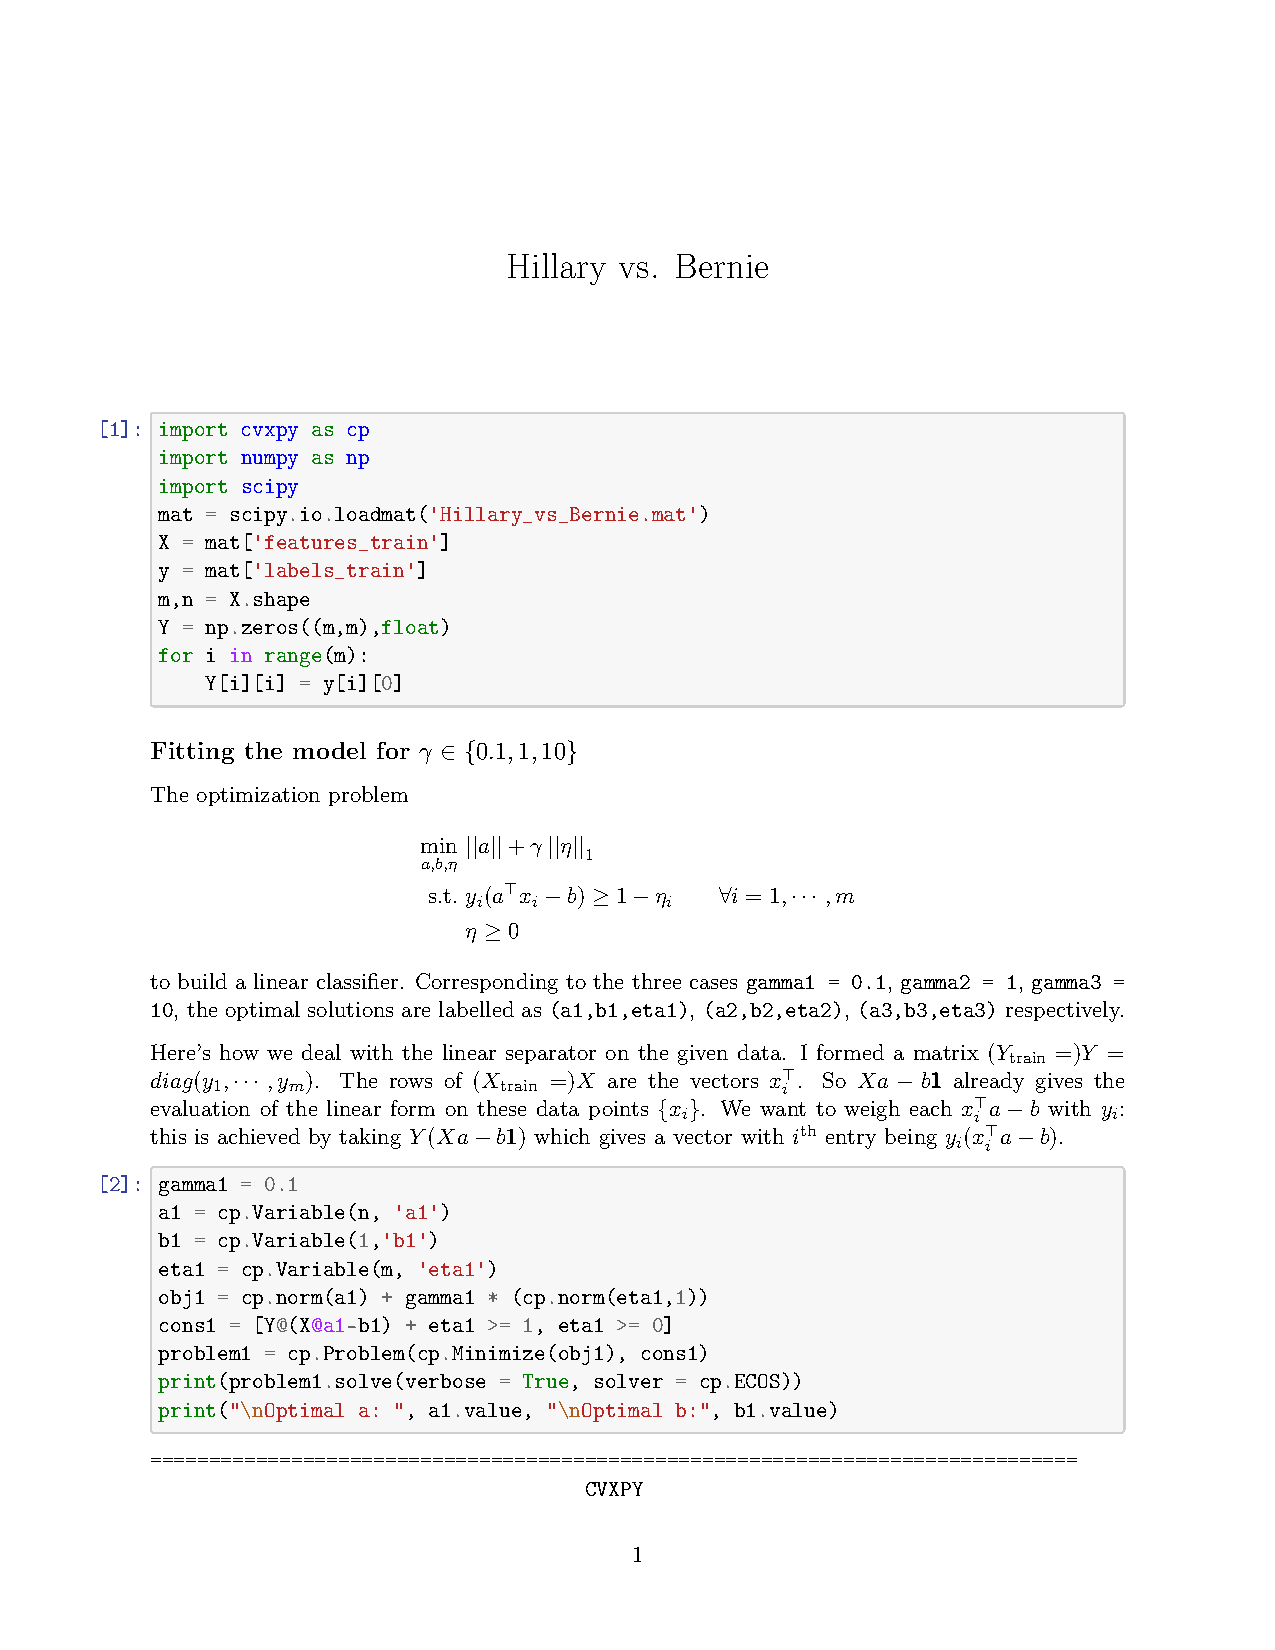
\includepdf[pages=-,pagecommand={\label{pdf:rad}}]{Hillary_vs_Bernie/Hillary Bernie.pdf}}





\end{document}

